\section{Loop Pipelining}
\label{bg:sec:loop_pipelining}

In this section, we explain the concept of loop pipelining, and how arithmetic
rules, when combined with other program transformations, can trade-off
accuracy, run time and resource utilization.

To start, we synthesize in Vivado HLS the following program in
Figure~\ref{bg:fig:dotprod} for calculating the dot-product, \verb|d|, of two
arrays, \verb|A| and \verb|B|, of single-precision floats bounded by $[0, 1]$.
\begin{figure}[ht]
\begin{lstlisting}
  float d = 0.0f;
  for (int i = 0; i < 1024; i++) {
      d = d + A[i] * B[i];
  }
\end{lstlisting}
    \caption{%
        A simple dot-product example which calculates the dot-product of two
        arrays \texttt{A} and \texttt{B}, each with 1024 elements.}
    \label{bg:fig:dotprod}
\end{figure}

Vivado HLS seek to optimize this loop by overlapping its iterations in a
process called pipelining.  By synthesizing this loop, we have obtained the
following schedule, in which iterations are laid out in rows, each clock cycle
is a column, \textbf{mul} and \textbf{add} are multiplication and addition
respectively, \verb|A[0]| and \verb|B[0]| are reads from the two arrays, and
the arrows indicate the data flow of \verb|d| across iterations, as shown in
Figure~\ref{bg:fig:sample_schedule_before}.
\begin{figure}[ht]
    \centering
    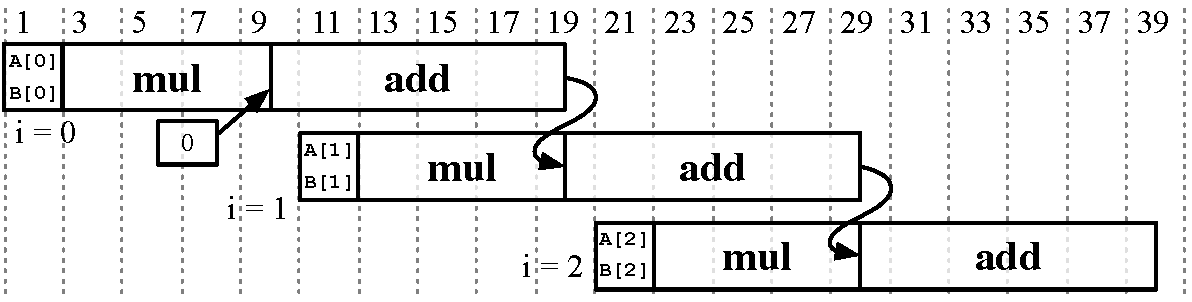
\includegraphics[width=0.8\linewidth]{sample_schedule_before}
    \caption{The resulting schedule of the example program in generated}
    \label{bg:fig:sample_schedule_before}
\end{figure}

Here we see that each iteration requires $18$ cycles, this value is known as
the \emph{depth}, $D$, of the loop.  Because in each iteration, we must wait
for the addition from previous iteration to complete before reading the value
of \verb|d|, \emph{data dependences} exist across iterations.  For this reason,
there are $10$ cycles between the starts of consecutive loop iterations, as
enforced by the data dependences, this value is known as the \emph{initiation
interval}.  Finally, the loop runs for $1024$ iterations (the \emph{trip
count}, $N$), so its overall latency is $((N-1)\times \II) + D = 10250$ cycles.

\begin{figure}[ht]
\begin{lstlisting}
  float d = 0.0f;
  for (int i = 0; i < 1024; i += 2) {
      d = (d + A[i]*B[i]) + A[i+1]*B[i+1];
  }
\end{lstlisting}
    \caption{Partially unrolled version of the original dot-product example.}
    \label{bg:fig:dotprod_unroll}
\end{figure}
Observe that the trip count can be halved by partial unrolling, as shown in
Figure~\ref{bg:fig:dotprod_unroll}.  Since we did not change data-paths by
unrolling, the data dependences remain unchanged, the resulting schedule
and the total latency stay the same.  However, by further exploiting the
associativity of addition, we can delay reading \verb|d| until later in each
iteration (Figure~\ref{bg:fig:dotprod_optimized}).
\begin{figure}[ht]
\begin{lstlisting}
  float d = 0.0f;
  for (int i = 0; i < 1024; i += 2) {
      d = d + (A[i]*B[i] + A[i+1]*B[i+1]);
  }
\end{lstlisting}
    \caption{Partially unrolled code optimized by applying associativity.}
    \label{bg:fig:dotprod_optimized}
\end{figure}

The program now admits the schedule in
Figure~\ref{bg:fig:sample_schedule_after}, which yields a loop latency
of $((512-1)\times 10) + 30 = 5140$ cycles---roughly half the original
latency. This optimized program, which is discovered automatically by our tool,
also reduces round-off errors by 50\% (as a result of the round-off errors
being accumulated in a different order) but increases LUT count by about 35\%
(because more operations are performed in each iteration).

\begin{figure}[ht]
    \centering
    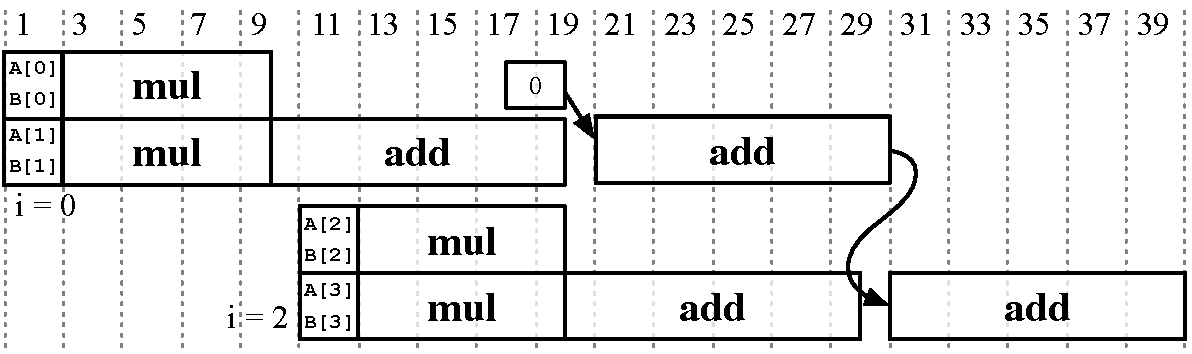
\includegraphics[width=0.8\linewidth]{sample_schedule_after}
    \caption{%
        The resulting schedule of the optimized code in
        Figure~\ref{bg:fig:dotprod_optimized}.}
    \label{bg:fig:sample_schedule_after}
\end{figure}

To accurately analyze the run time of a loop in a numerical program, it is
necessary to generate the schedule of the loop.  Algorithms for this, however,
tend to be computationally expensive, and exacerbated by the fact that we
need to apply this algorithm to each rewritten loops that we have discovered
using transformation rules.  For this we make use of the first few steps of a
scheduling technique known as \emph{iterative modulo scheduling}~\cite{rau94},
to efficiently compute a lower bound on the initiation interval as an
approximation to the actual value, and subsequently, the estimated run time of
the loop.
